\documentclass{article}

\usepackage{graphicx}
\usepackage{fullpage}


\graphicspath{ {img/} }
\begin{document}

\title{Program 4 Design and Analysis}
\author{Julian Brackins, Ryan Feather, Joe Mowry \and Charles Bonn}
\date{12/9/2014}
\maketitle

\section{Part 1 - Shared Memory}

\subsection{Program Description}

\subsection{Design}
Following Foster's design methodology, we have a brief overview:

\subsubsection{Partitioning}
        \begin{itemize}
            \item Reading values to be hashed
            \item Hashing
            \item Sending
            \item Recieving
            \item Inserting
        \end{itemize}
\subsubsection{Communication}
        \begin{itemize}
            \item Sharing data between computations
            \item Determine amount and pattern of communication
        \end{itemize}
\subsubsection{Aglomeration}
        \begin{itemize}
            \item Combine or group tasks to improve performance
        \end{itemize}
\subsubsection{Mapping}
        \begin{itemize}
            \item Assign agglomerated tasks to threads/physical processors.
        \end{itemize}


\subsection{Performance Testing}
\begin{figure}
  \caption{Timing Evaluation of increasing problem size}
  \centering
  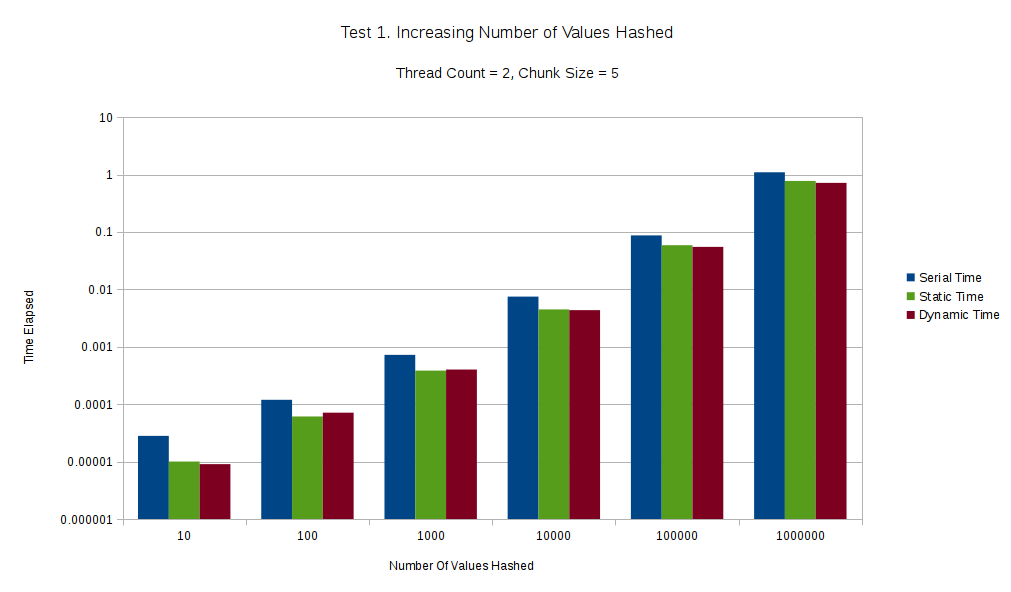
\includegraphics[width=\textwidth]{chart1a}
\end{figure}

\begin{figure}
  \caption{Speedup / Efficiency Evaluation of increasing problem size}
  \centering
  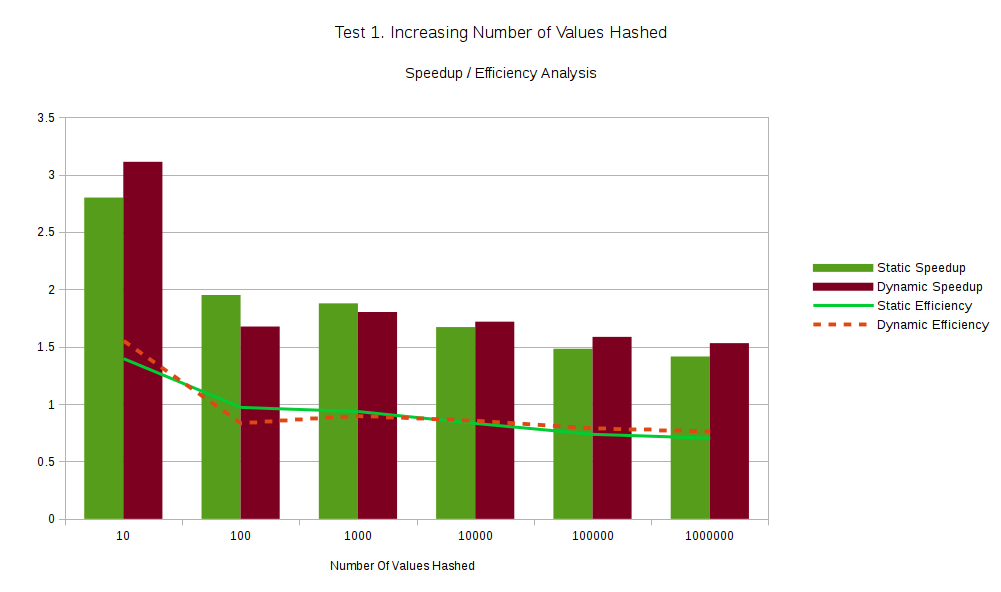
\includegraphics[width=\textwidth]{chart1b}
\end{figure}

\begin{figure}
  \caption{Timing Evaluation of increasing thread count}
  \centering
  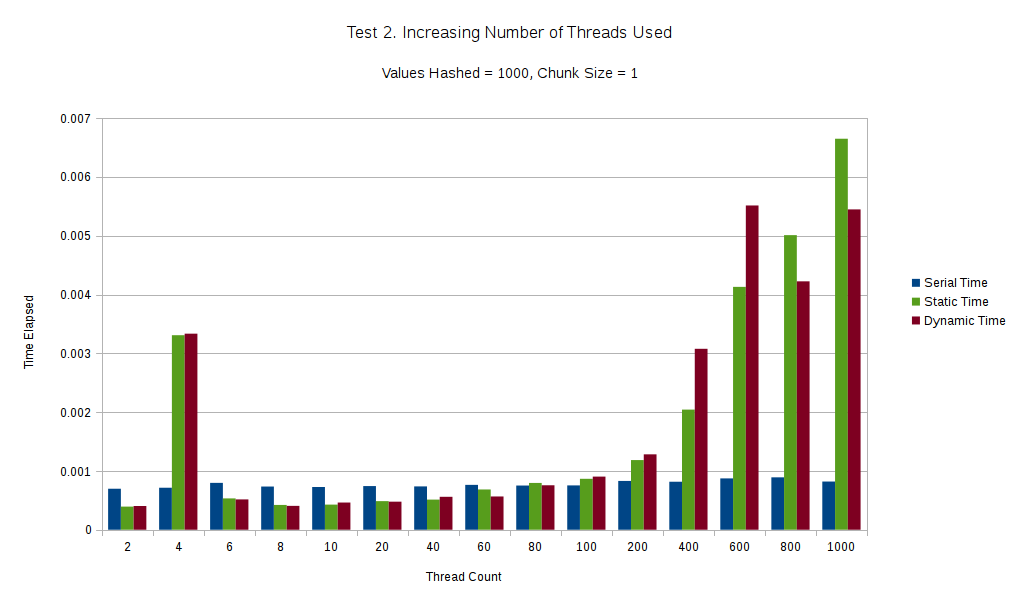
\includegraphics[width=\textwidth]{chart2a}
\end{figure}

\begin{figure}
  \caption{Speedup / Efficiency Evaluation of increasing thread count}
  \centering
  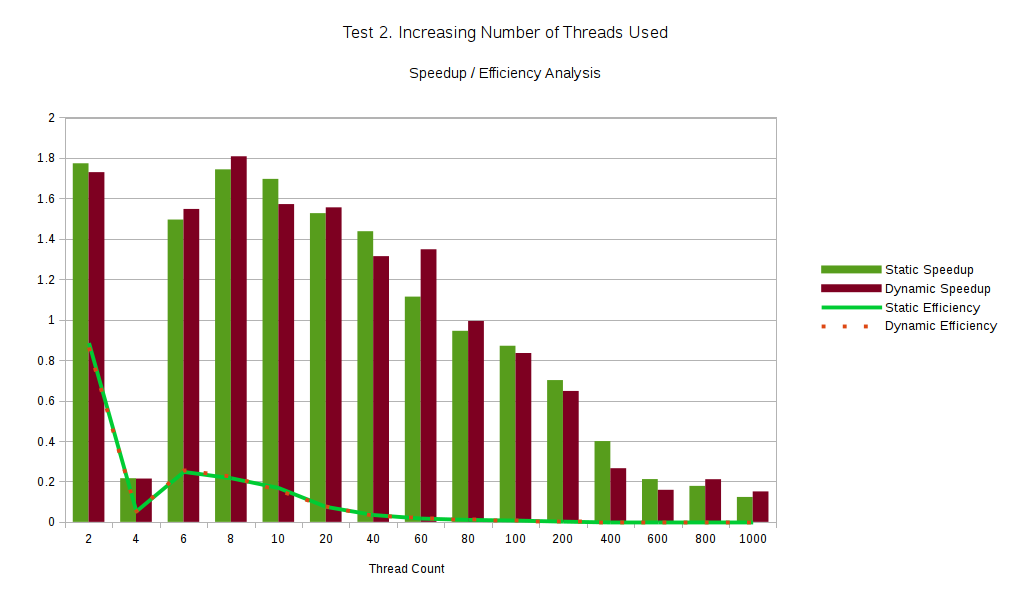
\includegraphics[width=\textwidth]{chart2b}
\end{figure}

\begin{figure}
  \caption{Timing Evaluation of increasing chunk size}
  \centering
  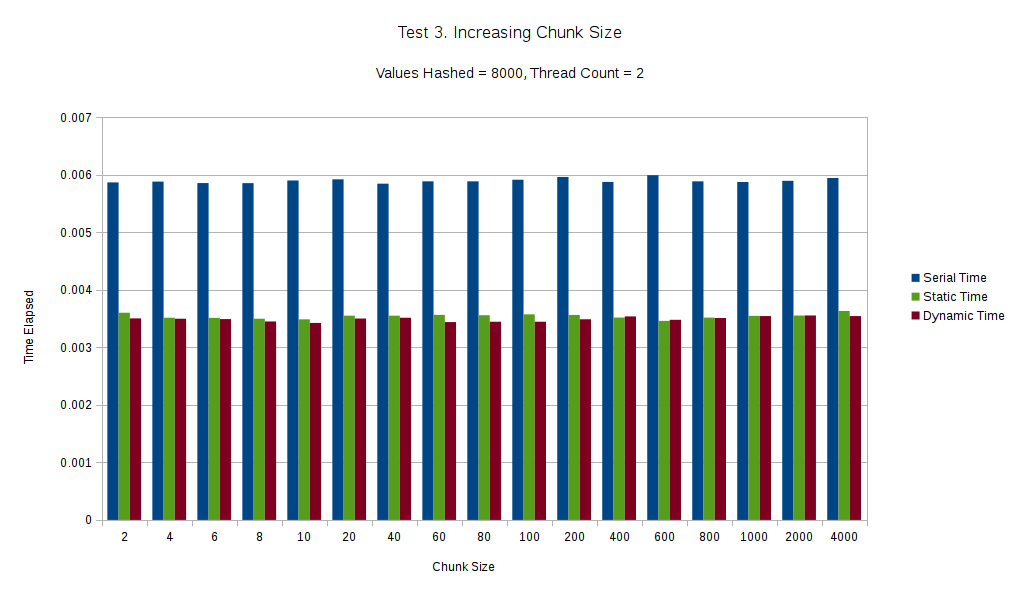
\includegraphics[width=\textwidth]{chart3a}
\end{figure}

\begin{figure}
  \caption{Speedup / Efficiency Evaluation of increasing chunk size}
  \centering
  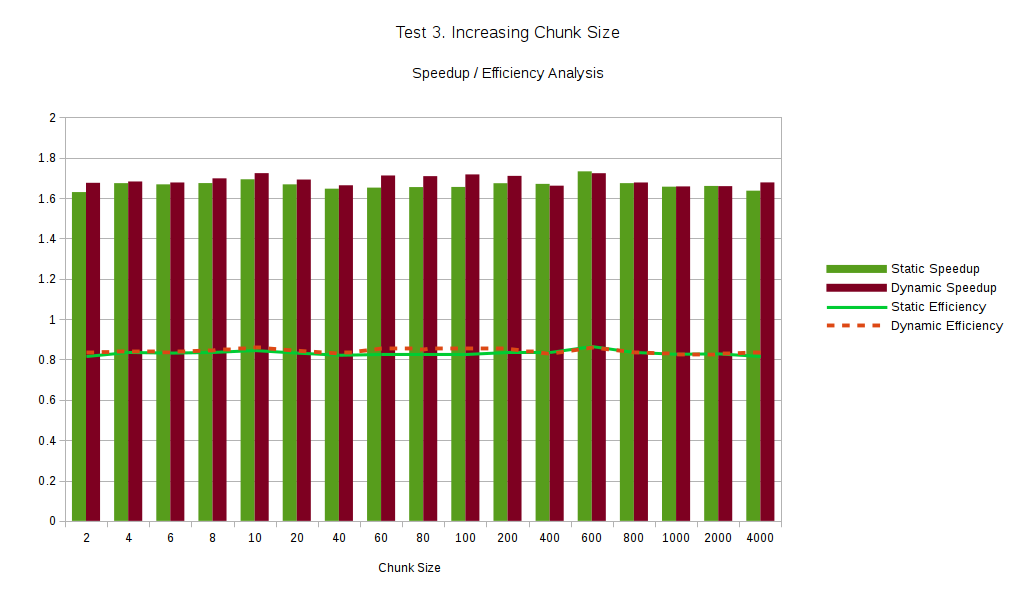
\includegraphics[width=\textwidth]{chart3b}
\end{figure}


\section{Part 2 - Distributed memory}
\subsection{Program Description}
This distributed memory program will allow for the typical hash table operations, but on a set of programs on potentially different computers.

Each process on each machine will be responsible for its own hash table, and respond to messages from a managing producer thread. The managing thread will give values to store and request table lookups.

The data is currently random strings read in from a file. A few sample inputs are provided.

\subsection{Design}
Following Foster's design methodology, we have a brief overview:

\subsubsection{Partitioning}
For our distributed memory solution, as in our shared, we will be doing data-centric partitioning. We will assign to each piece of data (in this case the strings) the tasks of hashing that data and storing it into a table. 

This will create a large number of tasks, much larger than our number of processors. There are no redundant computations, and each tak will be roughly the same size.

\subsubsection{Communication}
For each piece of data, in order to place it in a table, it must first be hashed according to the hash function. This is an example of local communication. Therfore, since the tasks are dependent, we can consolidate them into one single task, hashing and storing a value.

In addition, the tasks associated with a piece of data will work very independently. Very little global communication will be needed.

Communication is balanced, minimized, and all tasks can be performed concurrently.

\subsubsection{Aglomeration}
As discussed in the last section, each piece of data can be consolidated into one combined operation.

Other than that, there is not much agglomeration that can be done. Because the work associated with each piece of data is independint of the solution as a whole, and the locality of the table insert is minimal, we cannot group together tasks in a meaningful or advantageous way.

\subsubsection{Mapping}
For the distributed memory solution, we will employ a producer-consumer structure. We will have one root thread that produces values from an input file, handing out the values to the consumer threads. Each consumer thread will take the piece of data, hash it, and place it in the table.

It is very important that we balance the load that each consumer thread experiences, making sure that they are not overwhelemed with data that will make computation take longer or potentially fill up their table. At the same time, we want to make sure that the storing of data is determinstic, that way we can find the data in a later loopup operation. In order to do this, the data is hashed twice. Once by the root producer thread in order to determine which worker thread will get the data, and again by the worker to determine where in its table to place the data.



\subsection{Performance Testing}





\end{document}
